\documentclass[a4paper]{article}
\usepackage[x11names,svgnames]{xcolor}
\usepackage[T1]{fontenc}
\usepackage[utf8]{inputenc}
\usepackage[francais]{babel}
\usepackage{amsmath}
\usepackage{graphicx}
\usepackage{subfigure}
\usepackage[colorinlistoftodos]{todonotes}
\usepackage{array}
\usepackage{setspace}
\usepackage{fullpage}
\usepackage[justification=centering]{caption} % necessaire pour caption longue de plus d'une ligne.
\usepackage{hyperref} 
%\pdfcompresslevel=9 
\hypersetup{ 
     colorlinks=true, %colorise les liens 
     breaklinks=true, %permet le retour àˆ la ligne dans les liens trop longs 
     urlcolor= blue,  %couleur des hyperliens 
     linkcolor= Blue4, %couleur des liens internes crééŽs, 
}
\usepackage{listings}
\lstset{
language=python,
commentstyle=\textit,
basicstyle=\ttfamily\color{Black},
keywordstyle=\color{DarkRed},
commentstyle=\color{Blue3}\normalfont,
}
\newcommand{\cin}[1]{\lstinline{#1}}

% Francisation
\addto\captionsfrench{\renewcommand{\tablename}{{\scshape Tab.}}}

% Colonnes de largeur fixe
\newcolumntype{L}[1]{>{\raggedright\let\newline\\\arraybackslash\hspace{0pt}}m{#1}}
\newcolumntype{C}[1]{>{\centering\let\newline\\\arraybackslash\hspace{0pt}}m{#1}}
\newcolumntype{R}[1]{>{\raggedleft\let\newline\\\arraybackslash\hspace{0pt}}m{#1}}


\def\thesection{Question \arabic{section}}
\def\thesubsection{\alph{subsection}}

\onehalfspacing

% Bibliographie
\bibliographystyle{ieeetr}


\title{TP3 - IMN530}

\author{FOUQUET, Jérémie et MÉTHOT, Vincent}

\date{28 avril 2014}

\begin{document}
\maketitle

\section{IRM fonctionnelle \label{fmri}}

Plusieurs outils d'analyse existent déjà pour traiter des données d'IRMf. Nous avons choisis de les utiliser directement plutôt que de les implémenter en python. Deux suites logicielles ont retenu notre intérêt (puisque nous les connaissions déjà), soit FSL [http://fsl.fmrib.ox.ac.uk/fsl/fslwiki/] et AFNI [http://afni.nimh.nih.gov/], qu'il faudra avoir installé pour faire fonctionner le script associé à ce numéro (\lstinline{Q1\_IRMf.sh}).

\subsection{Étapes de reconstruction}

Il faut garder à l'esprit qu'à chaque étape de reconstruction, il est fortement conseillé d'inspecter visuellement les données. Dès leur réception, on a visuellement inspecté plusieurs tranches de \emph{fmri.nii} à tous les temps pour s'assurer que les artéfacts n'étaient pas trop important et que la correction de mouvement n'était pas nécessaire (voir Fig. \ref{fmri_anatomist}), comme mentionné dans la question. De plus, nous avons effectué une transformée de Fourier des séries temporelles (voir Fig. \ref{fmri_fft}).

\begin{figure}
   \centering
   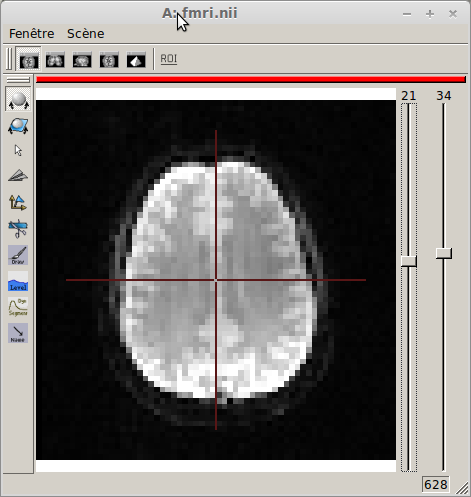
\includegraphics[width=.7\textwidth]{fmri_anatomist}
   \caption{\label{fmri_anatomist} Inspection visuelle de fmri.nii dans anatomist. On peut inspecter plusieurs tranches pour tous les points temporels à l'aide des deux curseurs à droite, comme dans un film.}
\end{figure}

\begin{figure}
   \centering
   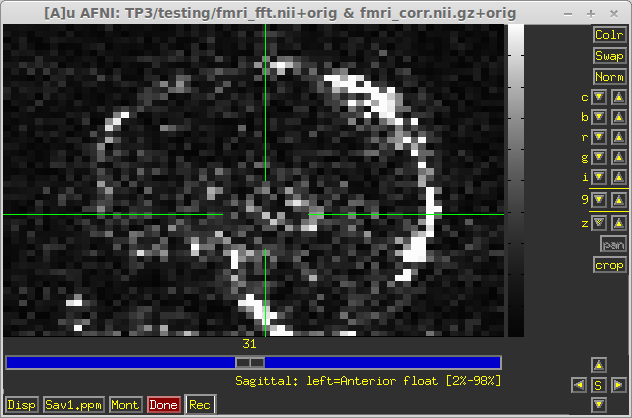
\includegraphics[width=.7\textwidth]{fmri_fft}
      \caption{\label{fmri_fft} Coupe sagitale de la transformée de Fourier de fmri.nii à chaque point. Une fréquence près de 0.02 Hz (la fréquence fondamentale du stimulus) est affichée dans AFNI. Les zones blanches peuvent être dues à de l'activation cérébrale mais aussi (et surtout) à un effet de bord relié à du mouvement.}
\end{figure}

Les étapes de reconstruction suivantes furent appliquées sur les données d'IRMf. Le résultat de chacune est illustrée sur la Fig. \ref{fmri_reconstruction}. On y voit sur la première ligne l'image originale (\ref{fmri_reconstruction}A - \emph{fmri.nii}) et les séries temporelles de quelques voxels voisins (\ref{fmri_reconstruction}B). Sur la deuxième ligne, il y a le résultat de la première étape de reconstruction ( \ref{fmri_reconstruction} A \& B \emph{fmri\_smooth.nii.gz}), c'est-à-dire l'image débruitée. Cette étape a pour but d'augmenter le rapport signal sur bruit par une convolution avec une gaussienne de FWHM = 6mm.
% Il y aurait avantage à utiliser un filtrage bilatéral, ou quelque chose de plus poussé...
La troisième ligne montre le résultat du filtrage temporel sur chaque voxel (\ref{fmri_reconstruction}E \emph{fmri\_low.nii.gz}). On voit par le fait même que la valeur moyenne de chaque voxel est fixée à 0, ne laissant que les variations temporelles. Comme du bruit et des artéfacts de nature physiologique se retrouvent aux hautes fréquences, nous avous décidé de couper les fréquences supérieures à 0.06 Hz (sachant que notre signal idéal à un fréquence fondamentale de 0.02 Hz) de chacune de nos séries temporelles (\ref{fmri_reconstruction}F).
La dernière étape de reconstruction consiste à calculer voxel par voxel une corrélation entre le signal idéal (contenu dans le fichier \emph{Data/ideal.txt}) et mesuré.  On en tire une carte de coefficients de corrélation entre -1 et 1 (\ref{fmri_reconstruction}F). On pourra ensuite seuiller cette carte pour obtenir un masque binaire des zones d'activations. La comparaison entre \ref{fmri_reconstruction}B et \ref{fmri_reconstruction}H montre l'effet du processus de reconstruction sur les données d'IRMf aurant au niveau spatial que temporel.

\begin{figure}
   \centering
   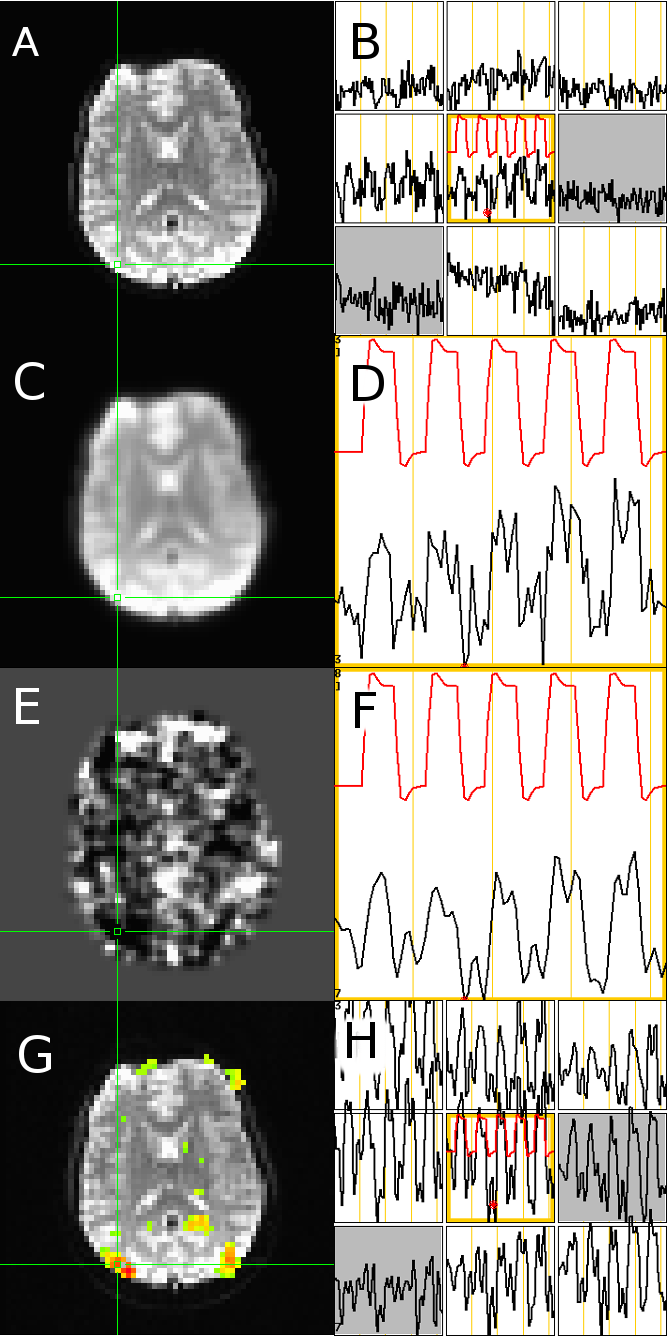
\includegraphics[height=0.85\textheight]{fmri_reconstruction}
      \caption{\label{fmri_reconstruction} A - Image originelle. B - Séries temporelles pour quelques voxels adjacents de l'image originelle. C - Image débruitée spatialement (convolution avec une gaussienne de FWHM = 6mm). D - Série temporelle débruitée. E - Image après passage d'une filtre passe-bas temporel. La valeur moyenne (fréquence nulle) représentant l'information structurelle est perdue. F - Série temporelle de l'image filtrée. G - Corrélation point à point (seuillé à $\rho > 0.5$). H - Séries temporelles pour quelques voxels adjacents de l'image reconstruite. Position du point sélectionné: x = 22, y = 13, z = 24. Les séries temporelles rouges représentent le signal idéal. Celles en noir représentent le signal mesuré/transformé.}
\end{figure}


\subsection{Segmentation \label{fmri_seg}}

On a effectué la segmentation des zones d'activation à l'aide de l'outil graphique d'AFNI, de manière à trouver les paramètres idéaux en fonction des zones que l'on s'attendait à voir activées. Puisque la tâche Roland est une tâche requérant des fonctions motrices, de mémoire et de vision, on s'attend à voir \og allumer \fg~ 6 zones reliées à ces activités. Les tâches motrices sont principalement localisées dans le cortex moteur (gyrus précentral). La mémoire est principalement localisée dans l'hippocampe. La vision est principalement localisée dans le cortex occipital. Nous nous sommes donc servis de nos connaissances anatomiques \emph{a priori} pour réaliser la segmentation et le regroupement des voxels activés (\emph{clustering}).

L'étape de segmentation dans le script \lstinline{Q1\_IRMf.sh} réalise l'opération de seuillage et de regroupement automatiquement. Elle donne sept régions distinctes, chacune d'entre elles étant étiquetée avec une valeur différente:
	
\begin{enumerate}
    \item Lobe occipital droit (vision)
    \item Lobe occipital gauche (vision)
    \item Hippocampe gauche (mémoire)
    \item Hippocampe droit (mémoire)
    \item Gyrus précentral droite (mouvement)
    \item Région hors du cerveau (artéfact)
    \item Gyrus précentral gauche (mouvement)
\end{enumerate}

La méthode de segmentation utilisée consiste en un seuillage simple des valeurs de coefficient de corrélation (on ne garde que celles entre 0.5149 et 1), puis le \emph{clustering} de AFNI enlève les voxels n'étant pas regroupés. Plus précisément, les groupes comportant moins de 50 voxels voisins sont mis à zéro.

\subsection{Zones d'activation}

On retrouve sur la Fig. \ref{fmri_2d} une projection des zones d'activation. On remarque en bas les zones visuelles (gauche et droite) et au centre les zones motrices (gauche et droite). Les zones reliées à la mémoire ne sont pas affichées par soucis de clarté de l'image. L'hippocampe gauche est toutefois visible sur la Fig. \ref{fmri_3d}, une capture d'écran 3d des zones d'activation. La région isolée à l'avant du cerveau n'est qu'un artéfact. On a créé ces deux images dans le fibernavigator.

\begin{figure}
\begin{center}
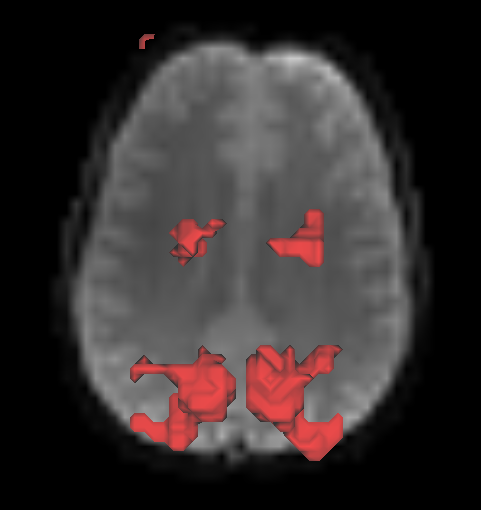
\includegraphics[width=0.6\textwidth]{fmri_2d}
\caption{Projection 2d des zones d'activation reconstruites dans le fibernavigator. En bas, zones visuelles gauche et droite. Au centre, zones motrices gauche et droite. Les hippocampes ne sont pas affichées pas soucis de clarté de l'image.
\label{fmri_2d}}
\end{center}
\end{figure}

\begin{figure}
\begin{center}
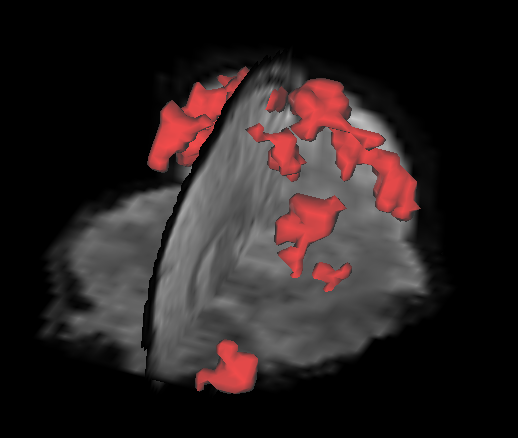
\includegraphics[width=0.6\textwidth]{fmri_3d}
\caption{Capture d'écran 3d des zones d'activation reconstruites dans le fibernavigator. En bas, artéfact de la reconstruction. Comparée à l'image de la Fig.\ref{fmri_2d}, on voit apparaître l'hippocampe gauche (la région la plus au centre).
\label{fmri_3d}}
\end{center}
\end{figure}

\section{IRM de diffusion}

\subsection{Estimation des tenseurs}
La fonction \lstinline{Q2_IRMd.tenseur} utilise la méthode de la pseudo-inverse pour effectuer le calcul des tenseurs. Elle peut prendre en entrée un masque qui indique pour quels voxels calculer les tenseurs. Sont également mis à 0 tous les éléments de tenseurs qui:
\begin{enumerate}
\item Correspondent à un signal à $b=0$ nul.
\item Prennent une valeur NaN ou Inf. 
\end{enumerate}
La fig. \ref{tenseurs_fiber} illustre les tenseurs que nous avons ainsi obtenus sur une carte de FA (calculée grâce à l'alogrithme présenté dans la section suivante).
\begin{figure}
\begin{center}
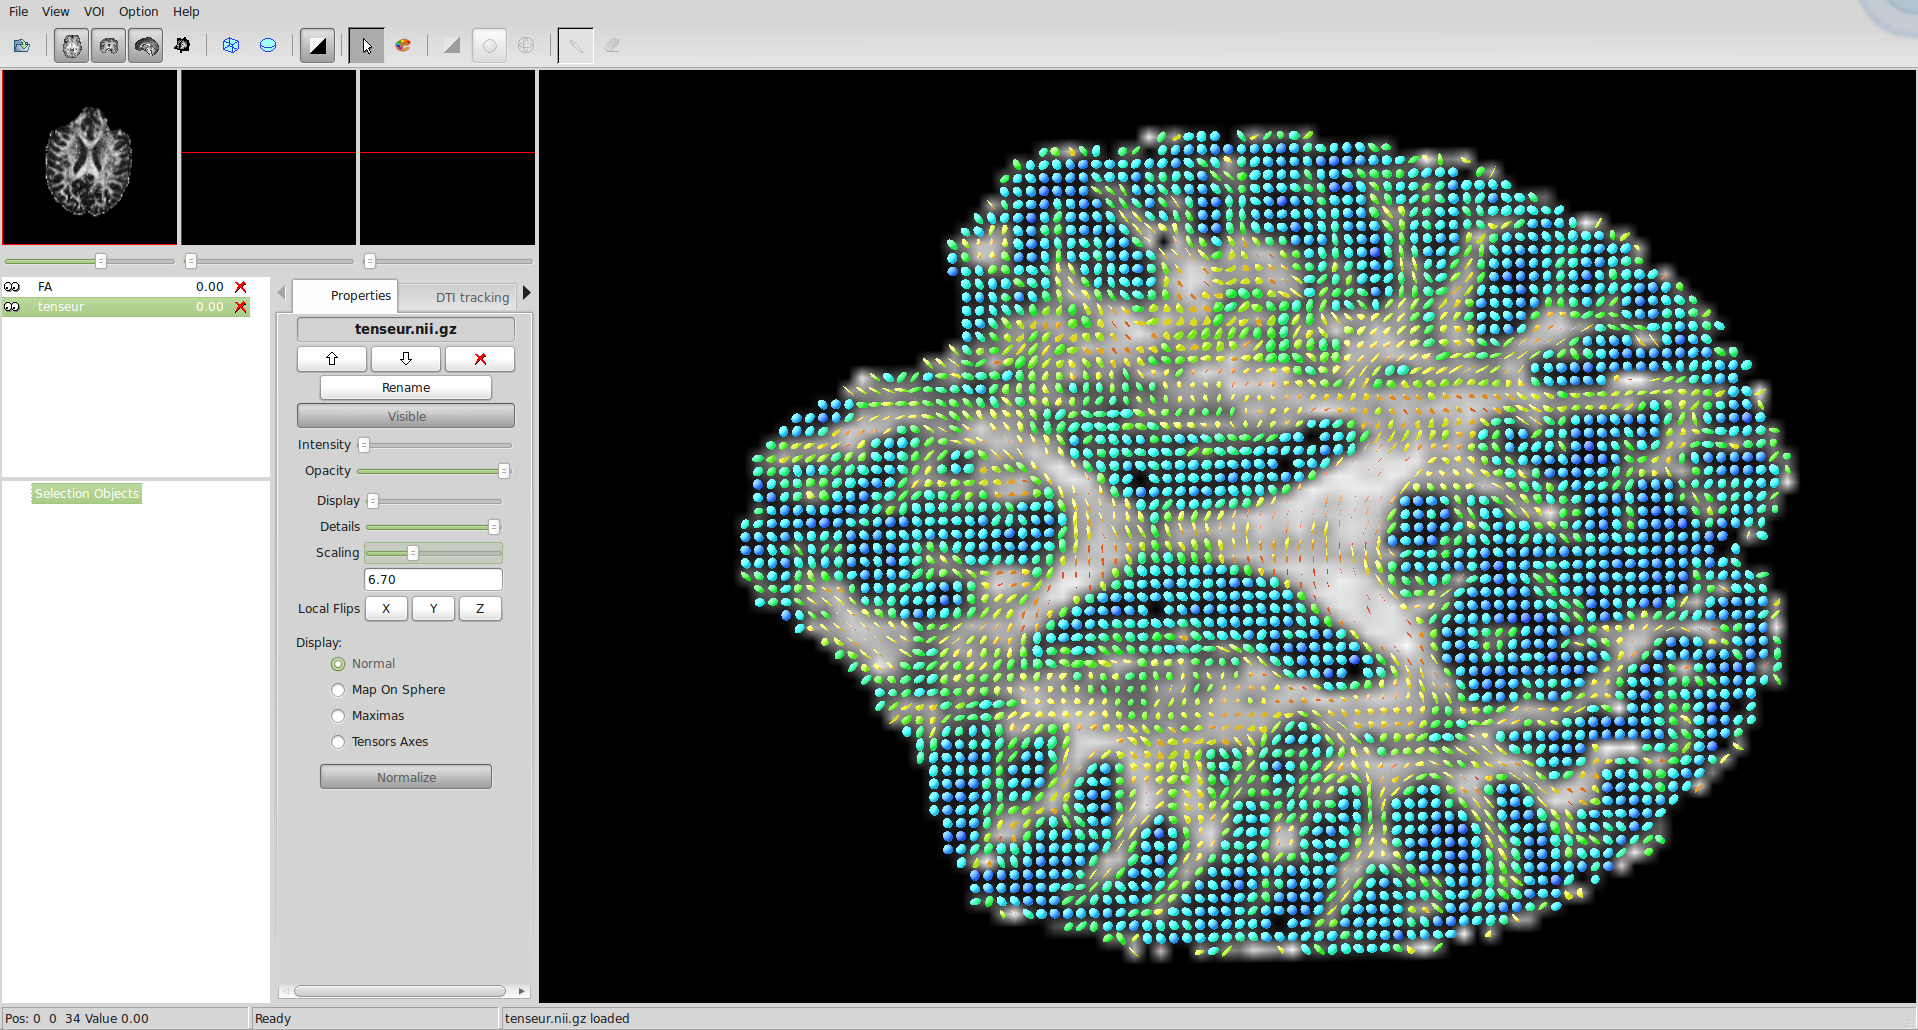
\includegraphics[scale=0.22]{tenseurs_fiber}
\caption{Illustration dans le Fibernavigator des tenseurs que nous avons obtenus grâce à la fonction \lstinline{Q2_IRMd.tenseur}. Les tenseurs sont superposés à la FA. À noter que seule une région identifiée comme étant le cerveau grâce à l'algorithme \lstinline{BET} de FSL est présentée. \label{tenseurs_fiber}}
\end{center}
\end{figure}

\subsection{FA et ADC}
La fonction \lstinline{Q2_IRMd.compAdcAndFa} calcule l'ADC et la FA à partir d'un champ de tenseur tel que calculé par la fonction \lstinline{Q2_IRMd.tenseur}. La fig. \ref{adc_fa} illustre pour certaines tranches l'ADC et la FA, respectivement. Les unités de l'ADC sont les mêmes que celles du coefficients de diffusion, soit $[longueur]^2/[temps]$, alors que la FA est sans unité.

\begin{figure}
\begin{center}
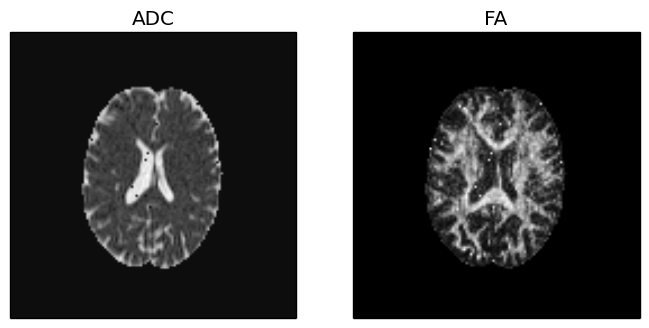
\includegraphics[scale=0.9]{adc_fa}
\caption{ADC et FA pour une tranche axiale du volume d'IRMd.\label{adc_fa}}
\end{center}
\end{figure}

\subsection{Tractographie}
La fonction \lstinline{Q2_IRMd.tracking} effectue une tractographie déterministe sur un champ de tenseurs. Les paragraphes suivants expliquent quelques enjeux importants de cette fonction.

\paragraph{À quelle étape interpoler?} Tout d'abord, lors de l'implémentation de la tractographie, nous avons dû prendre une décision concernant la question suivante: \textit{quel champ doit être interpolé à chaque pas de la tractographie?} Nous avons considéré les options présentées dans le tab. \ref{tracto_interp}. Ces options ont toutes des avantages et des inconvénients: plus le nombres d'éléments à interpoler et le nombre de calculs à faire avant d'arriver à une direction de propagation sont grands, plus le temps de calcul total de l'algorithme sera grand. Cependant, comme on le voit dans le tab. \ref{tracto_interp}, la précision possible du résultat final augmente aussi lorsque ces nombres augmentent. Il en est ainsi car en général, ce qui permet d'interpoler moins d'éléments génère une perte d'information précédant l'interpolation (les transformées effectuées ne sont en effet pas réversibles). Les interpolations faites par la suite risquent donc d'être moins précises. Nous avons choisi une méthode qui semblait être un compromis entre temps de calcul et précision possible, soit \textbf{l'interpolation des tenseurs}. Nous n'avons cependant pas eu le temps de tester l'impact réel sur les temps de calcul et la précision des résultats.

\begin{table}
\begin{center}
\begin{tabular}{C{.3\textwidth}|C{.1\textwidth}|C{.1\textwidth}|C{.15\textwidth}|C{.15\textwidth}}
\textbf{Champ interpolé} & \textbf{Nb d'interp.} & \textbf{Nb de calculs} & \textbf{Vitesse de calcul}  & \textbf{Précision possible}\\ \hline
Mesures d'IRMd & 64 & 3 & \textcolor{red}{Basse} & \textcolor{green}{Haute} \\
Tenseurs avant (après) décomposition & 6 & 2 (1)& \textcolor{yellow}{Moyenne} & \textcolor{yellow}{Moyenne} \\
Direction du vecteur principal & 2 & 0 & \textcolor{green}{Haute} & \textcolor{red}{Basse}
\end{tabular}
\end{center}
\caption{Champs pouvant être interpolés lors d'un pas de tractographie, avec le nombre d'éléments devant être interpolés pour chacun d'entre eux (colonne 2) ainsi que le nombre de calculs manquants avant d'arriver à une direction de propagation (colonne 3). Plus ces nombres sont grands, plus le temps de calcul est grand. Cependant, en descendant dans les rangées du tableau, de l'information est également perdue avant l'interpolation. Ceci pourrait rendre l'interpolation moins précise. \label{tracto_interp}}
\end{table}

\paragraph{Méthode d'interpolation} La méthode d'interpolation a un impact crucial sur la vitesse de notre algorithme. Nous avons essayé les méthodes: plus proche voisin, linéaire et spline de degré $n$, avec $n$ allant de 2 à 5. Avec une méthode plus complexe que la méthode linéaire, l'interpolation devenait très visiblement le goulot d'étranglement de la vitesse de notre algorithme. Cependant, cela n'a pas causé d'amélioration apparente de la qualité de notre tractographie. Les autres résultats présentés dans ce rapport ont donc été obtenus avec avec la méthode d'interpolation linéaire. 

\paragraph{Résultats} La figure \ref{tracking} illustrent des fibres obtenues pour différents pas et différents seuil sur la FA, avec 10000 graines placées aléatoirement.

\begin{figure}
\begin{center}
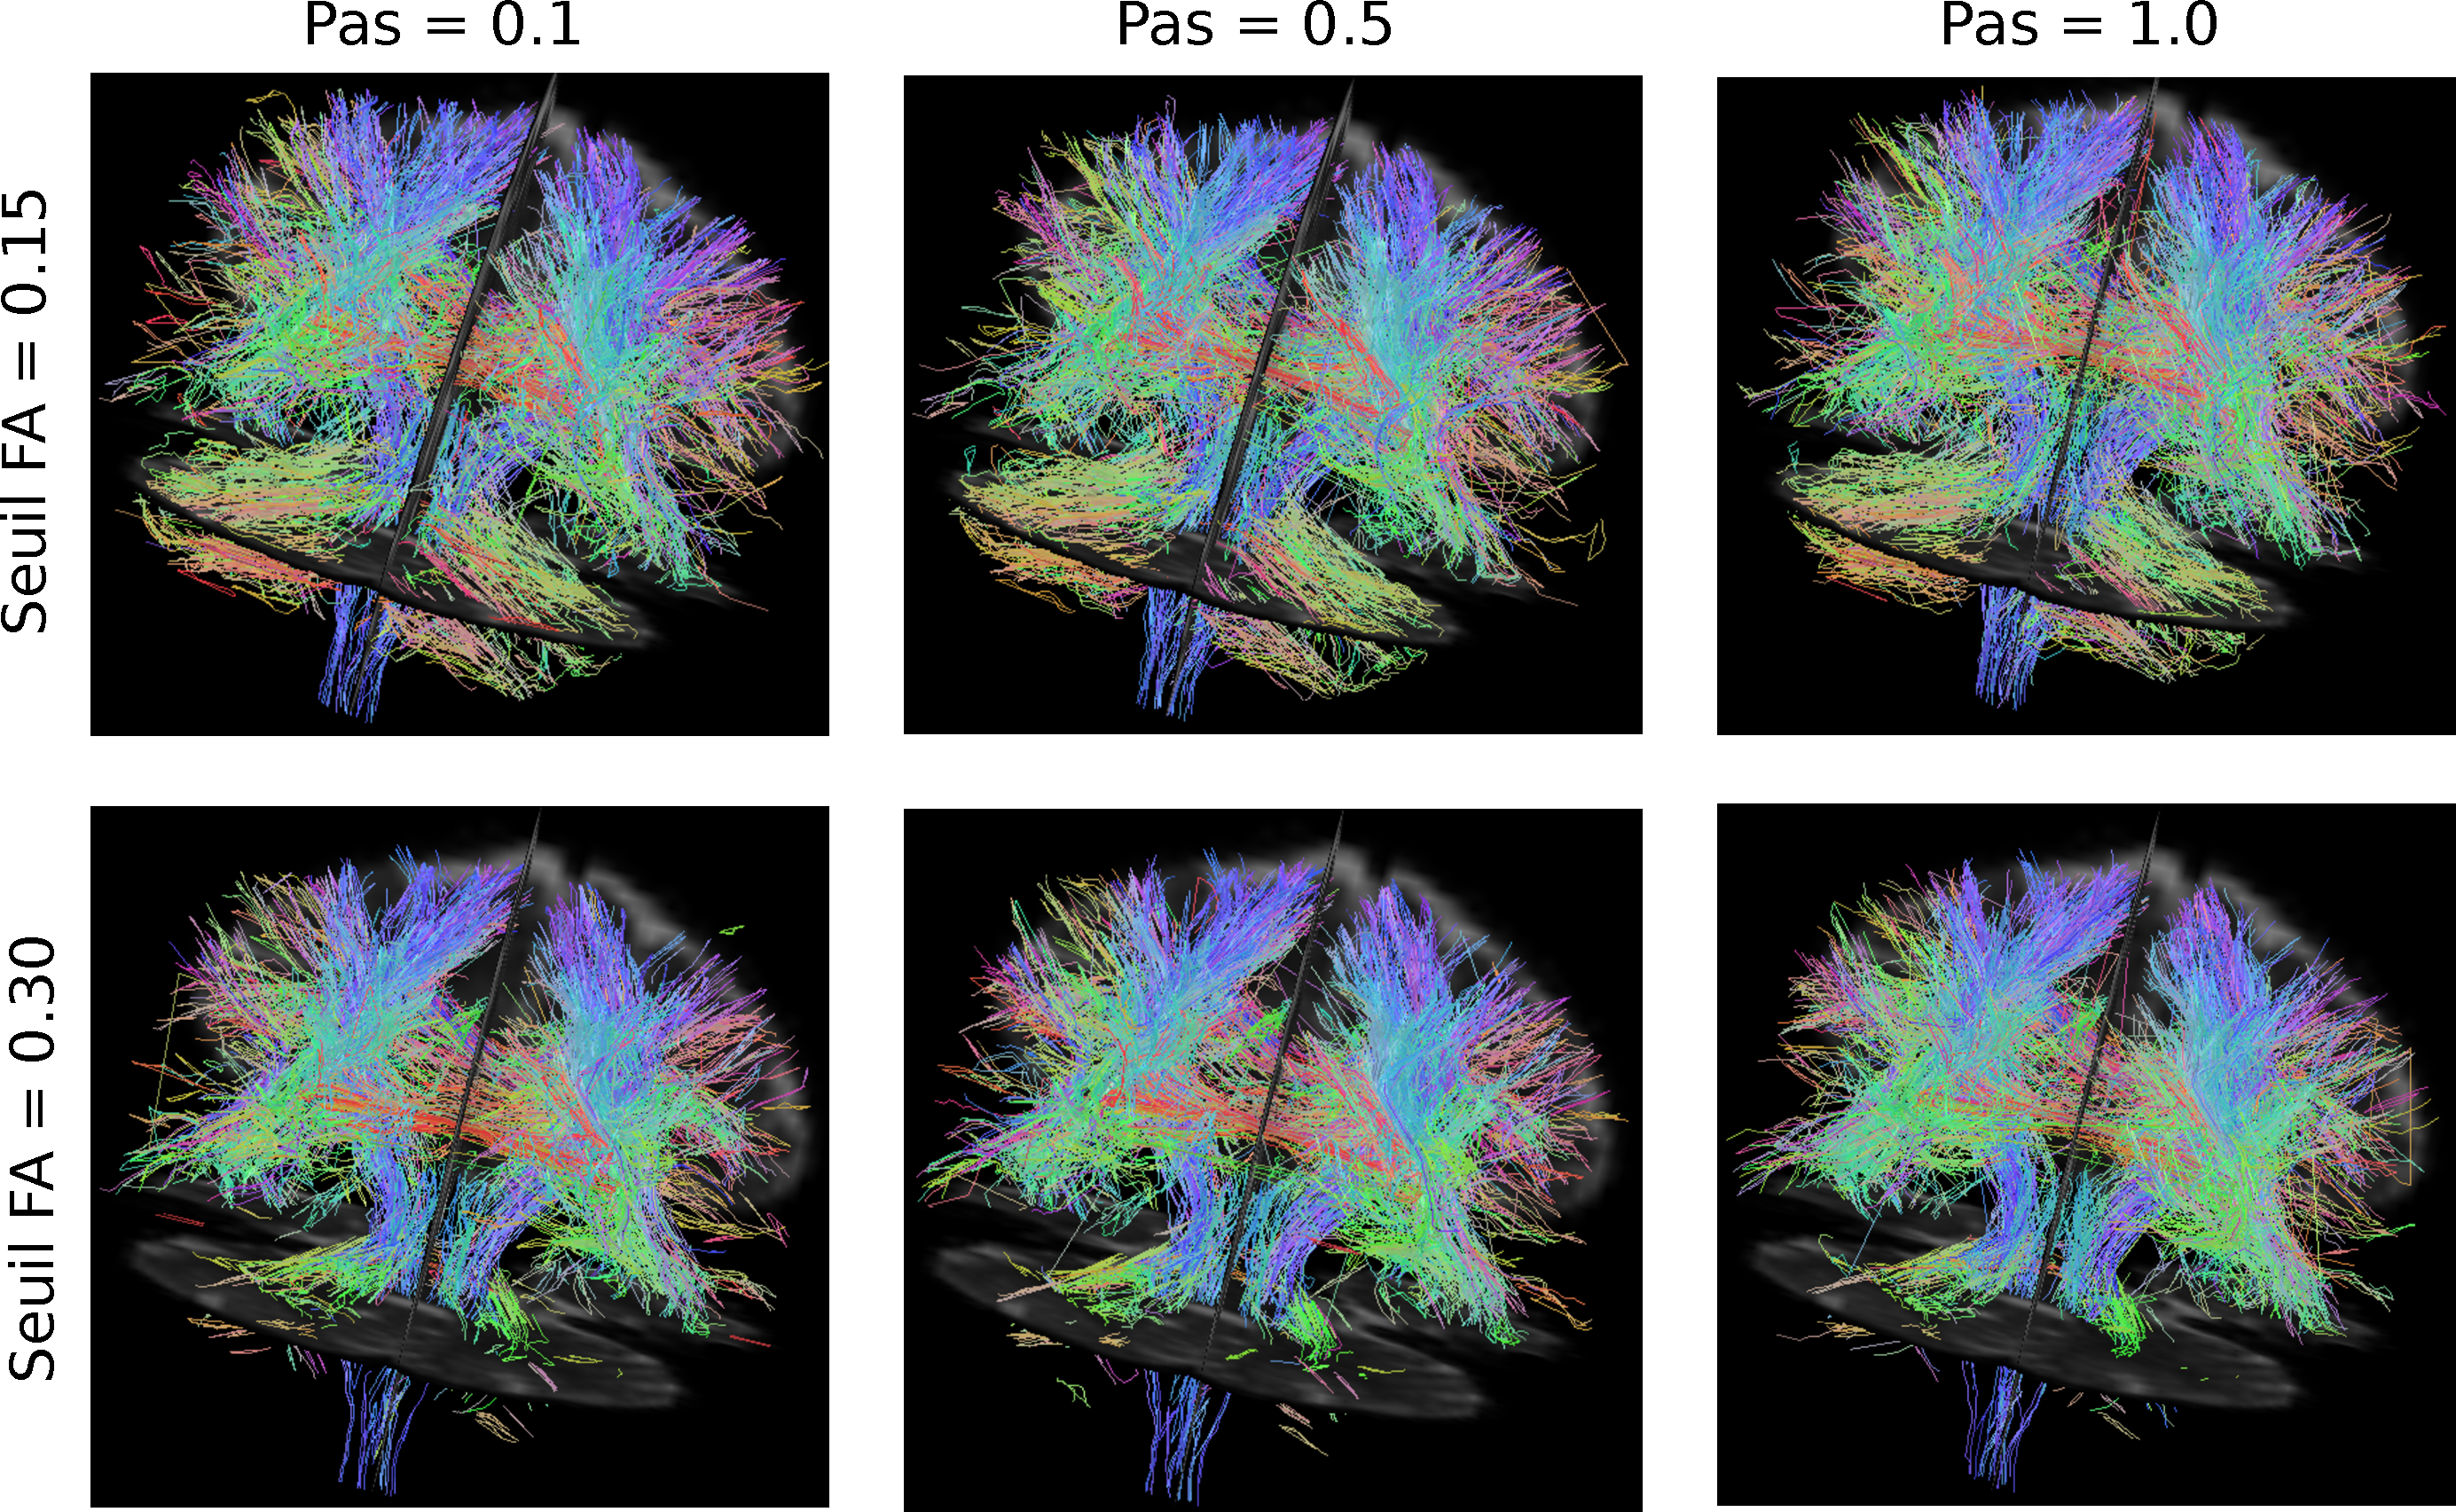
\includegraphics[scale=.3]{tracking}
\caption{Fibres obtenues avec 10000 graines placées aléatoirement pour différentes valeurs de pas et de seuil sur la FA visualisées dans le Fibernavigator et superposées à l'image à $b=0$. On voit bien une augmentation du nombre et de la longueur des fibres lorsque le seuil diminue. Cela est particulièrement visible dans le cervelet. Le pas ne semble pour sa part pas avoir une influence majeure sur l'apparence des fibres. \label{tracking}}
\end{center}
\end{figure}

\section{Fusion}

\subsection{Justification}
\paragraph{Espace de recalage}Pour choisir l'espace de référence dans lequel effectuer les recalages, nous avons cherché l'espace de l'image qui détenait
\begin{enumerate}
\item La meilleure résolution
\item Le moins d'artéfacts
\item Le plus haut SNR
\end{enumerate}
Nous voulions en effet recaler les images sur celle qui représentait le plus fidèlement et le plus précisément la réalité, ce qui était reflété par ces caractristiques. L'espace choisi a donc évidemment été l'espace de l'image T1.

\paragraph{Outil}
Tout d'abord, mentionnons que pour l'IRMd, nous avons recalé l'image à $b=0$ sur l'image T1, C'est en effet elle qui possédait le plus haut SNR et se rapprochait le plus d'une image anatomique habituelle. En IRMf, nous avons recalé la moyenne temporelle du signal sur l'image T1 afin de maximiser le SNR de l'image recalée. De plus, pour les deux volumes recalés, nous avons remarqué que le processus était grandement facilité si les cerveaux étaient \og extraits \fg~ avant le recalage. Nous avons donc appliqué la fonction \lstinline{fsl5.0-bet} sur tous les volumes avant le recalage, avec des paramètres permettant une bonne extraction du cerveau.

Ensuite, nous avons choisi le logiciel de recalage ANTS pour la grande variété des possibilités qu'il offre de même que pour sa réputation. Étant donné les différences importantes entre les pondérations des images recalées, les mesures de similarité que nous avons envisagées sont l'information mutuelle (IM) et la corrélation-croisée (CC). 

Pour recaler l'IRMd sur la T1, nous avons d'abord essayé une transformation affine (il est toujours bon d'essayer une méthode plus simple pour commencer). Les résultats étaient déjà relativement prometteurs, mais quelques éléments de l'image ne semblaient pas encore parfaitement recalés, peut-être en raison d'artéfacts (fig. \ref{b0-to-t1}). Nous avons donc essayé quelques combinaisons de recalage non-linéaire qu'offrait ANTS. Après inspection visuelle des résultats, nous avons subjectivement arrêté notre choix sur le recalage avec une CC de rayon 4, une transformation de type élastique avec un pas de gradient de 3, une régularisation gaussienne sur le gradient de la transformation de paramètres 0.5 et 3 et des nombres d'itérations de 30, 20 et 10 sur les échelles de résolution x/4, x/2 et x, avec x la résolution initiale (en langage ANTS, \lstinline{-m CC[...,1,4] -t Elast[3] -i 30x20x10 -r Gauss[0.5,3]}. Les résultats sont illustrés sur la fig. \ref{b0-to-t1}.
\begin{figure}
\begin{center}
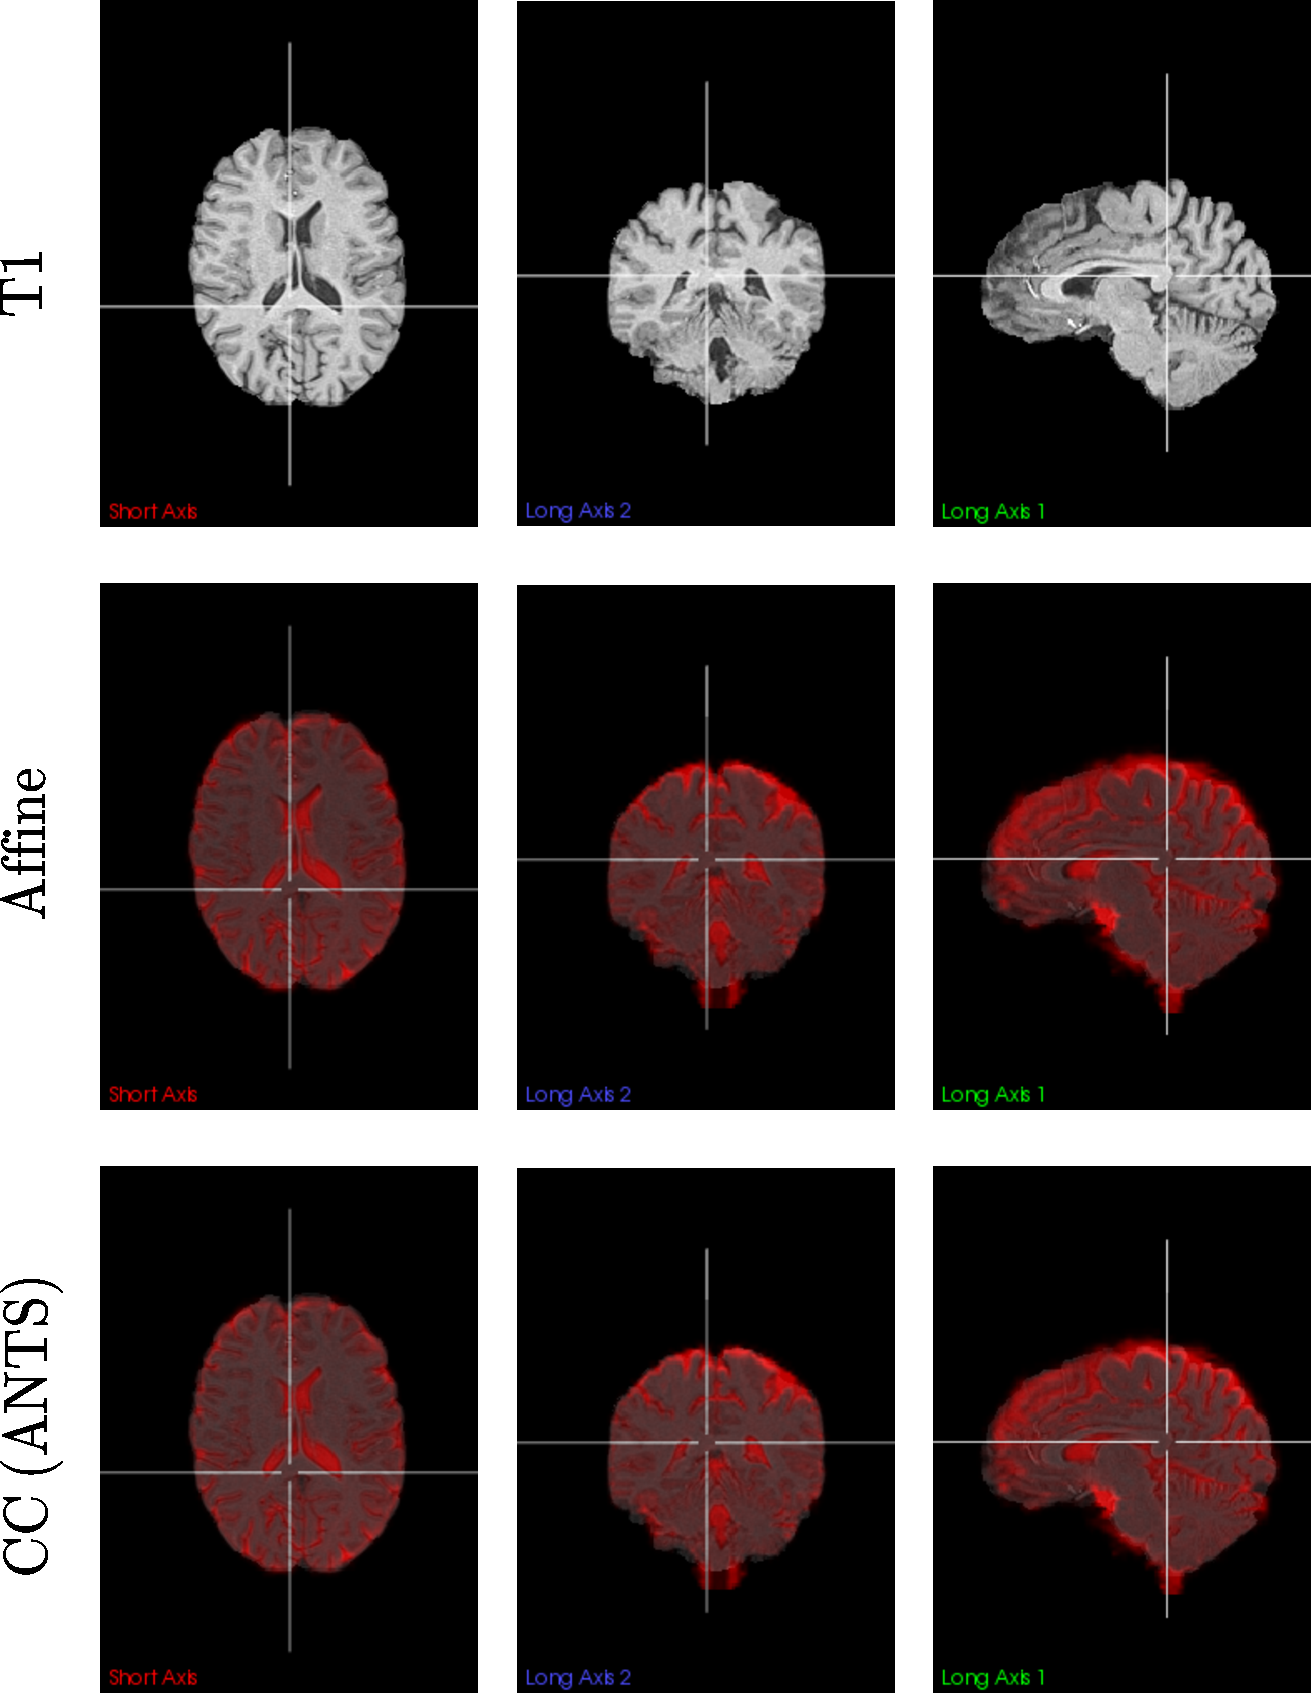
\includegraphics[scale=0.5]{b0-to-t1}
\caption{Recalage de l'image d'IRMd à $b=0$ (en rouge) sur l'image T1 à l'aide d'une transformation affine (ligne 2) et d'une transformation non linéaire avec ANTS utilisant les paramètres suivants en langage ANTS: \lstinline{-m CC[...,1,4] -t Elast[3] -i 30x20x10 -r Gauss[0.5,3]}. \label{b0-to-t1}}
\end{center}
\end{figure}  

Pour recaler l'IRMf sur la T1, nous avons utiliser la même approche que pour l'IRMd. L'image d'IRMf présentait cependant une résolution spatiale encore plus faible que l'IRMd, et son SNR semblait aussi assez faible. Il était donc plus difficile de qualifier le recalage. Nous avons finalement arrêté notre choix sur la même méthode de recalage non linéaire que pour l'IRMd. Les résultats sont illustrés sur la fig. \ref{fmri-to-t1}

\begin{figure}
\begin{center}
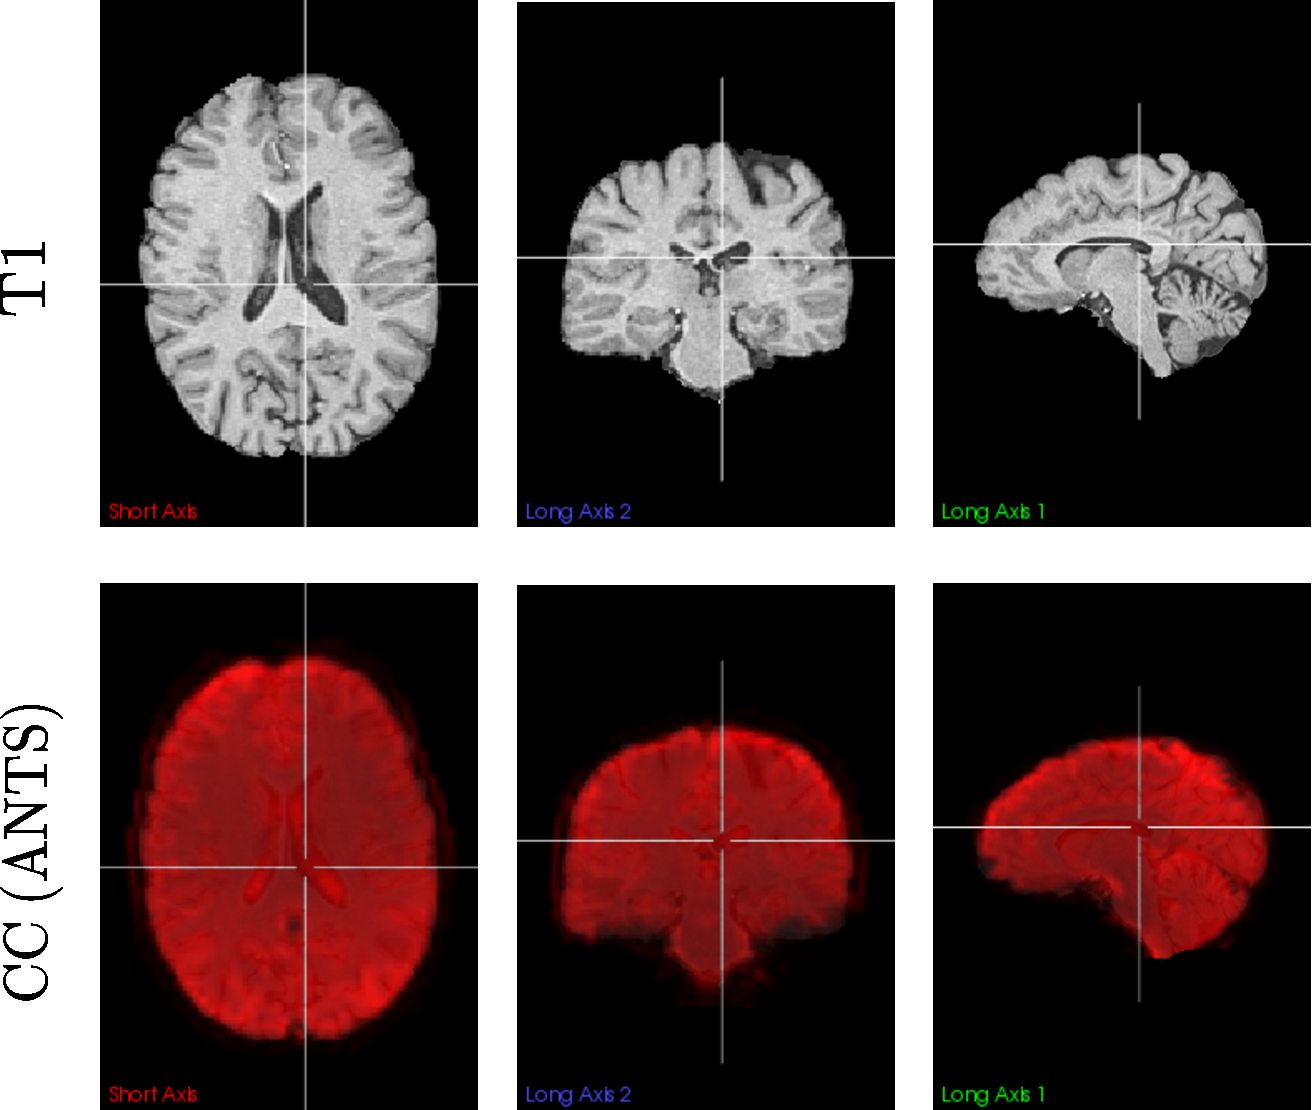
\includegraphics[scale=0.5]{fmri-to-t1}
\caption{Image T1 (rangée 1) et recalage non linéaire de l'image d'IRMf moyennée dans le temps (en rouge, rangée 2) sur l'image T1 effectué avec ANTS avec les paramètres suivants, en langage ANTS: \lstinline{-m CC[...,1,4] -t Elast[3] -i 30x20x10 -r Gauss[0.5,3]}. \label{fmri-to-t1}}
\end{center}
\end{figure}  

\subsection{Connectivité des zones fonctionnelles}
Pour étudier la connectivité des zones fonctionnelles, nous avons chargé dans le Fibernavigator les tenseurs, les zones d'activation (en binaire) et l'image T1 après recalage. Toujours dans le Fibernavigator, nous ensuite avons lancé des tractographies déterministes avec des graines à la surface de chacune des zones d'activation identifiées dans la \ref{fmri_seg}. En plaçant les graines sur la surface d'une seule zone à la fois, il nous était possible de voir à quelles autres zones elle étaie connectée. Les réseaux de fibres ainsi obtenus sont présentés sur la fig. \ref{fusion_dti}. Les principaux paramètres de tractographie utilisés sont un seuil sur la matière blanche de 0.20, un angle maximal de $\pi/3$ et un pas de 1mm.

\begin{figure}
\begin{center}
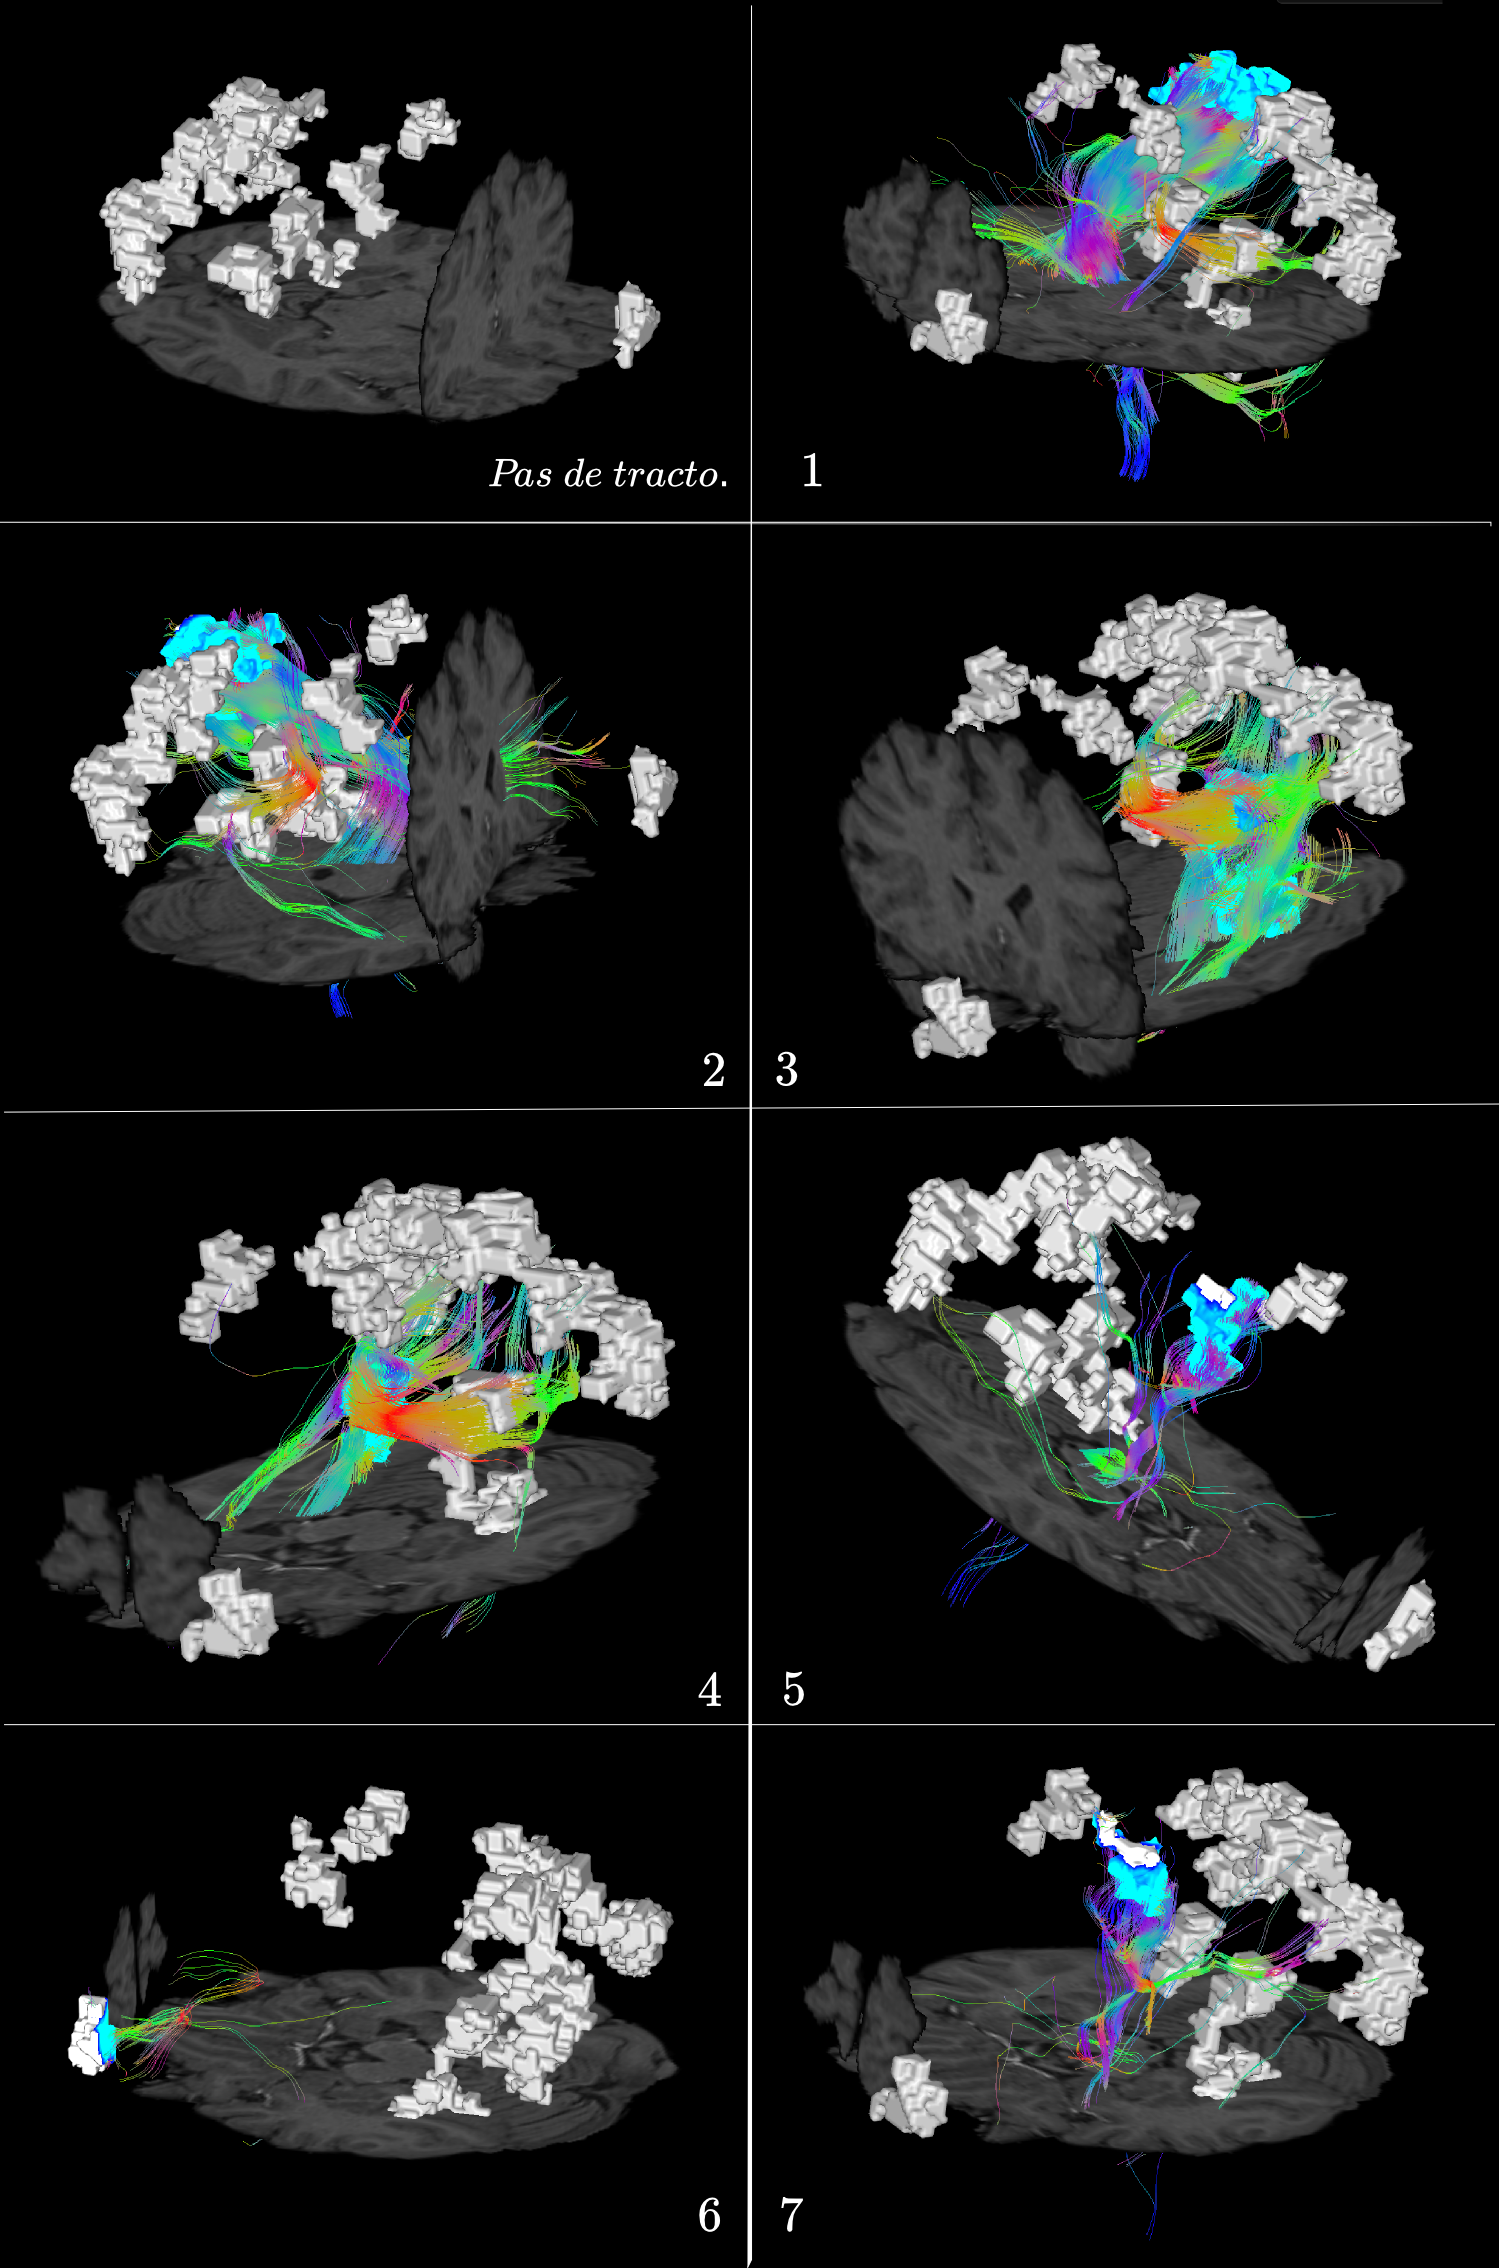
\includegraphics[height=.8\textheight]{fusion_dti}
\caption{Réseaux de fibres obtenus en plaçant des graines à la surface de chacune des zones d'activation identifiées à la \ref{fmri}. Les surfaces colorées (une par sous-image) sont les zones d'activation à partir desquelles la tractographie était lancée. Les surfaces blanches représentent toutes les autres zones d'activation. Les numéros des sous-images correspondent aux numéros des régions identifiées à la \ref{fmri}.\ref{fmri_seg}. 	\label{fusion_dti}}
\end{center}
\end{figure}

De façon qualitative, on remarque que les deux lobes occipitaux (région 1 et 2) sont connectés aux deux régions de l'hippocampe (région 3 et 4) de façon importante. Quelques fibres relient les lobes occipitaux entre eux, mais elles ne sont pas très nombreuses. Les deux régions de l'hipocampe semblent quant à elles fortement liées entre elles. Les gyrus précentraux (régions 5 et 7) ne semblent pas fortement connectés à d'autres régions activées, si ce n'est que légèrement à leur lobe occipital ipsilatéral. Comme nous pouvions nous y attendre, la région 6, qui était un artéfact, n'est reliée à aucune autre zone.

\section{Bonus}

\subsection{FA et ADC}

La FA est une mesure d'anisotropie du tenseur. Une FA de 0 représente un tenseur isotrope (une sphère) alors qu'une FA de 1 représente un tenseur complètement anisotropique dans une direction (un aiguille). Ainsi, on trouve ainsi une FA minimale de 0 dans les ventricules, où il n'y a aucune structure (et la diffusion est isotrope), alors qu'une FA maximale de 0.996 est visible dans le corps calleux, une struture très anisotrope.

Dans le corps calleux, les fibres sont majoritairement dans la même direction, et on y retrouve des valeurs de FA entre 0.65 et 0.996. Dans les zones de croisement de fibre, on observe une baisse de la FA (entre 0.4 et 0.6). Ceci s'explique par l'incapacité du tenseur à bien modéliser les croisements de fibre. Comme le calcul de la FA n'implique que l'amplitude de diffusion dans les trois directions principales, cette mesure se voit irrémédiablement réduire dans les zones de croisement.

L'ADC est une mesure effective du coefficient de diffusion. Lorsqu'elle est nulle, les molécules d'eau sont à l'arrêt. Plus elle est élevée, plus l'eau peut voyager loin en peu de temps. L'ADC possède ici des valeurs entre 0 et 0.0038 mm$^2$/sec (les unités inverses de la b-value) dont les plus basses se retrouvent un peu partout dans la matière blanche (très structurée) et la plus haute dans le liquide céphalo-rachidien. Les croisements ne semblent pas avoir d'impact sur l'ADC, qui est de l'ordre de 0.001 autant dans les zones de croisement que dans le corps calleux.

\subsection{Tractographie avec Dipy}
Pour effectuer la tractographie sur un champ de fODFs avec Dipy, nous avons tenté de suivre l'exemple \textit{Reconstruction with Constrained Spherical Deconvolution} présenté dans la documentation de Dipy en ligne [http://nipy.org/dipy/examples\_built/reconst\_csd.html\#example-reconst-csd].

Nous avons été capable d'effectuer une tractographie sur une partie de notre image d'IRMd de taille 20x20x20 (fig. \ref{} et script \lstinline{Q4_bonus.py}). Cependant, pour l'image IRMd complète, le temps de calcul du champ de fODF était de plus de 5 heures (le temps exact nous est en fait inconnu, car nous n'avons pas eu le temps d'attendre la fin du calcul).

Il resterait donc à optimiser le code ébauché pour accélérer les calculs (p. ex. parallélisation). Aussi, il serait possible d'essayer une tractographie avec un champ d'ODF demandant moins de temps de calcul que celui de l'exemple utilisé.


\end{document}